\section[Major Contribution 2]{Major Contribution 2: Distributed-memory multi-GPU block-sparse tensor contraction for electronic structure}

\begin{frame}[t]
  \frametitle{Electronic Structure Application}

  \begin{itemize}
  \item Accurate simulation of electronic structure
  \item Quantum Chemistry
  \item Coupled Cluster Singles and Doubles (CCSD)
    \begin{itemize}
    \item $O(n^6)$, $O(n^4)$ space. $n = O(\textrm{\# atoms})$
    \item $\Rightarrow$ a few (5-10) atoms on a workstation
    \item a few dozen (50-100) atoms on a supercomputer
    \end{itemize}
  \item fast/reduced scaling formulations $\Rightarrow$ 100s of atoms on a workstation
    \begin{itemize}
    \item Time to solution in days
    \item \textcolor{teal}{$\Rightarrow$ we should get time to solutions in minutes on a supercomputer}
    \end{itemize}
  \item Complex tensor algebra
  \item Single terms represents 90\% of computation:
  \end{itemize}

  $$
  R_{ab}^{ij} = \sum_{cd} T_{cd}^{ij}V_{ab}^{cd} + \ldots
  $$
  
\end{frame}

%% \begin{frame}[t]
%%   \frametitle{ABCD tensor product}

%%   \begin{center}
%%   \begin{tikzpicture}
%%     \node at (0,0) {$
%%       \tikzmarknode{R}{R}_{\tikzmarknode{ab}{ab}}^{\tikzmarknode{ij}{ij}} = \sum_{\tikzmarknode{cd}{cd}}
%%       \tikzmarknode{T}{T_{cd}^{ij}}\tikzmarknode{V}{V_{ab}^{cd}} + \ldots
%%       $};
%%     \draw[teal,-latex,line width=.5mm] (1,-2) node[below,teal] {Elements to be refined iteratively (typically 10-20 iterations)} .. controls (1,-1) and ([yshift=-1cm]T.south) .. (T.south);
%%     \draw[teal,-latex,line width=.5mm] (2.5,2) node[above,teal] {Fixed between iterations} .. controls (2.5,1) and ([yshift=1cm]V.north) .. (V.north);
%%     \draw[teal,-latex,line width=.5mm] (-3,0) node[left,teal] {Make vanish} -- (R.west);
%%     \draw[orange,-latex,line width=.5mm] (-2.5,1) node[above,orange] {M} .. controls (-2.5,0.5) and ([yshift=0.5cm]ij.north) .. (ij.north);
%%     \draw[orange,-latex,line width=.5mm] (-2.5,-1) node[below,orange] {N} .. controls (-2.5,-0.5) and ([yshift=-0.5cm]ab.south) .. (ab.south);
%%     \draw[orange,-latex,line width=.5mm] (-1,-1.25) node[below,orange] {K} .. controls (-1,-0.5) and ([yshift=-0.5cm]cd.south) .. (cd.south);
%%   \end{tikzpicture}
%%   \end{center}

%%   \begin{tikzpicture}[remember picture,overlay]
%%     \node[orange,xshift=-4cm,yshift=1.5cm,align=center] at (current page.south east) {
%%       $C_{m,n} \leftarrow C_{m,n} + A_{m, k}B_{k, n}$,\\
%%       with $m\in [1, M], n\in [1, N], k\in [1, K]$\\
%%       and $N = K >> M$};
%%   \end{tikzpicture}

%%   \begin{itemize}
%%   \item $i, j, a, b, c, d = O(n)$
%%   \item $i = j, a = b = c = d = [5, 20]i$
%%   \end{itemize}
%% \end{frame}

\begin{frame}[t]
  \frametitle{Block-Sparse Representation}

  \begin{columns}
    \begin{column}{0.5\textwidth}
    \resizebox{8cm}{!}{\begin{tikzpicture}[
        %Global config
        baseline=0cm,
        >={Stealth[length=7pt,width=13pt]},
        line width=.5pt,
        ampersand replacement=\&,
        %Styles
        Matrix/.style={
            matrix of nodes,
            font=\scriptsize,
            text height=1.5pt,
            text depth=1pt,
            text width=1.5pt,
            align=center,
            column sep=1.5pt,
            row sep=1.5pt,
            nodes in empty cells,
        },
    ]

    \matrix[Matrix] at (0,0) (B){ % Matrix contents 
        \& \& \& \& \& \& \& \& \& \&  \\
        \& \& \& \& \& \& \& \& \& \&\\
        \& \& \& \& \& \& \& \& \& \&  \\
        \& \& \& \& \& \& \& \& \& \&\\
        \& \& \& \& \& \& \& \& \& \&  \\
        \& \& \& \& \& \& \& \& \& \&\\
        \& \& \& \& \& \& \& \& \& \&  \\
        \& \& \& \& \& \& \& \& \& \&\\
        \& \& \& \& \& \& \& \& \& \&  \\
        \& \& \& \& \& \& \& \& \& \&\\
        \& \& \& \& \& \& \& \& \& \&  \\
    };

    \matrix[Matrix,below=2pt of B.south] (C){ % Matrix contents 
        \& \& \& \& \& \& \& \& \& \&\\
        \& \& \& \& \& \& \& \& \& \&\\
        \& \& \& \& \& \& \& \& \& \&\\
        \& \& \& \& \& \& \& \& \& \&\\
        \& \& \& \& \& \& \& \& \& \&\\
        \& \& \& \& \& \& \& \& \& \&\\
   };

    \matrix[Matrix,left=2pt of C.west] (A){ % Matrix contents 
        \& \& \& \& \& \& \& \& \& \&\\
        \& \& \& \& \& \& \& \& \& \&\\
        \& \& \& \& \& \& \& \& \& \&\\
        \& \& \& \& \& \& \& \& \& \&\\
        \& \& \& \& \& \& \& \& \& \&\\
        \& \& \& \& \& \& \& \& \& \&\\
   };

   \node[draw,fill=gray!25,inner sep=0,fit=(A-1-1)(A-1-1)](A00){};
   \node[draw,inner sep=0,fit=(A-2-1)(A-2-1)](A10){};
   \node[draw,fill=gray!25,inner sep=0,fit=(A-3-1)(A-4-1)](A20){};
   \node[draw,inner sep=0,fit=(A-5-1)(A-5-1)](A30){};
   \node[draw,fill=gray!25,inner sep=0,fit=(A-6-1)(A-6-1)](A40){};

   \node[draw,inner sep=0,fit=(A-1-2)(A-1-3)](A01){};
   \node[draw,fill=gray!25,inner sep=0,fit=(A-2-2)(A-2-3)](A11){};
   \node[draw,fill=gray!25,inner sep=0,fit=(A-3-2)(A-4-3)](A21){};
   \node[draw,fill=gray!25,inner sep=0,fit=(A-5-2)(A-5-3)](A31){};
   \node[draw,inner sep=0,fit=(A-6-2)(A-6-3)](A41){};

   \node[draw,fill=gray!25,inner sep=0,fit=(A-1-4)(A-1-6)](A02){};
   \node[draw,inner sep=0,fit=(A-2-4)(A-2-6)](A12){};
   \node[draw,fill=gray!25,inner sep=0,fit=(A-3-4)(A-4-6)](A22){};
   \node[draw,inner sep=0,fit=(A-5-4)(A-5-6)](A32){};
   \node[draw,inner sep=0,fit=(A-6-4)(A-6-6)](A42){};

   \node[draw,fill=gray!25,inner sep=0,fit=(A-1-7)(A-1-9)](A03){};
   \node[draw,fill=gray!25,inner sep=0,fit=(A-2-7)(A-2-9)](A13){};
   \node[draw,fill=gray!25,inner sep=0,fit=(A-3-7)(A-4-9)](A23){};
   \node[draw,fill=gray!25,inner sep=0,fit=(A-5-7)(A-5-9)](A33){};
   \node[draw,inner sep=0,fit=(A-6-7)(A-6-9)](A43){};

   \node[draw,inner sep=0,fit=(A-1-10)(A-1-10)](A04){};
   \node[draw,fill=gray!25,inner sep=0,fit=(A-2-10)(A-2-10)](A14){};
   \node[draw,fill=gray!25,inner sep=0,fit=(A-3-10)(A-4-10)](A24){};
   \node[draw,inner sep=0,fit=(A-5-10)(A-5-10)](A34){};
   \node[draw,fill=gray!25,inner sep=0,fit=(A-6-10)(A-6-10)](A44){};

   \node[draw,fill=gray!25,inner sep=0,fit=(A-1-11)(A-1-11)](A05){};
   \node[draw,inner sep=0,fit=(A-2-11)(A-2-11)](A15){};
   \node[draw,inner sep=0,fit=(A-3-11)(A-4-11)](A25){};
   \node[draw,fill=gray!25,inner sep=0,fit=(A-5-11)(A-5-11)](A35){};
   \node[draw,inner sep=0,fit=(A-6-11)(A-6-11)](A45){};

   \node[draw,fill=gray!25,inner sep=0,fit=(B-1-1)(B-1-2)](B00){};
   \node[draw,inner sep=0,fit=(B-2-1)(B-3-2)](B10){};
   \node[draw,fill=gray!25,inner sep=0,fit=(B-4-1)(B-6-2)](B20){};
   \node[draw,fill=gray!25,inner sep=0,fit=(B-7-1)(B-9-2)](B30){};
   \node[draw,inner sep=0,fit=(B-10-1)(B-10-2)](B40){};
   \node[draw,fill=gray!25,inner sep=0,fit=(B-11-1)(B-11-2)](B50){};

   \node[draw,inner sep=0,fit=(B-1-3)(B-1-5)](B01){};
   \node[draw,fill=gray!25,inner sep=0,fit=(B-2-3)(B-3-5)](B11){};
   \node[draw,inner sep=0,fit=(B-4-3)(B-6-5)](B21){};
   \node[draw,inner sep=0,fit=(B-7-3)(B-9-5)](B31){};
   \node[draw,fill=gray!25,inner sep=0,fit=(B-10-3)(B-10-5)](B41){};
   \node[draw,inner sep=0,fit=(B-11-3)(B-11-5)](B51){};

   \node[draw,inner sep=0,fit=(B-1-6)(B-1-7)](B02){};
   \node[draw,inner sep=0,fit=(B-2-6)(B-3-7)](B12){};
   \node[draw,fill=gray!25,inner sep=0,fit=(B-4-6)(B-6-7)](B22){};
   \node[draw,inner sep=0,fit=(B-7-6)(B-9-7)](B32){};
   \node[draw,fill=gray!25,inner sep=0,fit=(B-10-6)(B-10-7)](B42){};
   \node[draw,inner sep=0,fit=(B-11-6)(B-11-7)](B52){};

   \node[draw,inner sep=0,fit=(B-1-8)(B-1-9)](B03){};
   \node[draw,fill=gray!25,inner sep=0,fit=(B-2-8)(B-3-9)](B13){};
   \node[draw,inner sep=0,fit=(B-4-8)(B-6-9)](B23){};
   \node[draw,inner sep=0,fit=(B-7-8)(B-9-9)](B33){};
   \node[draw,fill=gray!25,inner sep=0,fit=(B-10-8)(B-10-9)](B43){};
   \node[draw,inner sep=0,fit=(B-11-8)(B-11-9)](B53){};

   \node[draw,inner sep=0,fit=(B-1-10)(B-1-10)](B04){};
   \node[draw,fill=gray!25,inner sep=0,fit=(B-2-10)(B-3-10)](B14){};
   \node[draw,fill=gray!25,inner sep=0,fit=(B-4-10)(B-6-10)](B24){};
   \node[draw,fill=gray!25,inner sep=0,fit=(B-7-10)(B-9-10)](B34){};
   \node[draw,inner sep=0,fit=(B-10-10)(B-10-10)](B44){};
   \node[draw,inner sep=0,fit=(B-11-10)(B-11-10)](B54){};

   \node[draw,fill=gray!25,inner sep=0,fit=(B-1-11)(B-1-11)](B05){};
   \node[draw,inner sep=0,fit=(B-2-11)(B-3-11)](B15){};
   \node[draw,fill=gray!25,inner sep=0,fit=(B-4-11)(B-6-11)](B25){};
   \node[draw,inner sep=0,fit=(B-7-11)(B-9-11)](B35){};
   \node[draw,inner sep=0,fit=(B-10-11)(B-10-11)](B45){};
   \node[draw,inner sep=0,fit=(B-11-11)(B-11-11)](B55){};

   \node[draw,fill=gray!25,inner sep=0,fit=(C-1-1)(C-1-2)](C00){};
   \node[draw,inner sep=0,fit=(C-2-1)(C-2-2)](C10){};
   \node[draw,fill=gray!25,inner sep=0,fit=(C-3-1)(C-4-2)](C20){};
   \node[draw,fill=gray!25,inner sep=0,fit=(C-5-1)(C-5-2)](C30){};
   \node[draw,fill=gray!25,inner sep=0,fit=(C-6-1)(C-6-2)](C40){};

   \node[draw,inner sep=0,fit=(C-1-3)(C-1-5)](C01){};
   \node[draw,fill=gray!25,inner sep=0,fit=(C-2-3)(C-2-5)](C11){};
   \node[draw,fill=gray!25,inner sep=0,fit=(C-3-3)(C-4-5)](C21){};
   \node[draw,fill=gray!25,inner sep=0,fit=(C-5-3)(C-5-5)](C31){};
   \node[draw,inner sep=0,fit=(C-6-3)(C-6-5)](C41){};

   \node[draw,fill=gray!25,inner sep=0,fit=(C-1-6)(C-1-7)](C02){};
   \node[draw,fill=gray!25,inner sep=0,fit=(C-2-6)(C-2-7)](C12){};
   \node[draw,fill=gray!25,inner sep=0,fit=(C-3-6)(C-4-7)](C22){};
   \node[draw,inner sep=0,fit=(C-5-6)(C-5-7)](C32){};
   \node[draw,fill=gray!25,inner sep=0,fit=(C-6-6)(C-6-7)](C42){};

   \node[draw,inner sep=0,fit=(C-1-8)(C-1-9)](C03){};
   \node[draw,fill=gray!25,inner sep=0,fit=(C-2-8)(C-2-9)](C13){};
   \node[draw,fill=gray!25,inner sep=0,fit=(C-3-8)(C-4-9)](C23){};
   \node[draw,fill=gray!25,inner sep=0,fit=(C-5-8)(C-5-9)](C33){};
   \node[draw,fill=gray!25,inner sep=0,fit=(C-6-8)(C-6-9)](C43){};

   \node[draw,fill=gray!25,inner sep=0,fit=(C-1-10)(C-1-10)](C04){};
   \node[draw,fill=gray!25,inner sep=0,fit=(C-2-10)(C-2-10)](C14){};
   \node[draw,fill=gray!25,inner sep=0,fit=(C-3-10)(C-4-10)](C24){};
   \node[draw,fill=gray!25,inner sep=0,fit=(C-5-10)(C-5-10)](C34){};
   \node[draw,inner sep=0,fit=(C-6-10)(C-6-10)](C44){};

   \node[draw,fill=gray!25,inner sep=0,fit=(C-1-11)(C-1-11)](C05){};
   \node[draw,inner sep=0,fit=(C-2-11)(C-2-11)](C15){};
   \node[draw,fill=gray!25,inner sep=0,fit=(C-3-11)(C-4-11)](C25){};
   \node[draw,inner sep=0,fit=(C-5-11)(C-5-11)](C35){};
   \node[draw,fill=gray!25,inner sep=0,fit=(C-6-11)(C-6-11)](C45){};

   \path[left] (A00.north west) -- node (l2) {$p_0$} (A00.south west);
   \path[left] (A10.north west) -- node {$p_1$} (A10.south west);
   \path[left] (A20.north west) -- node {$p_0$} (A20.south west);
   \path[left] (A30.north west) -- node {$p_1$} (A30.south west);
   \path[left] (A40.north west) -- node (l3) {$p_0$} (A40.south west);

   \path[above] (A00.north west) -- node (l4) {$q_0$} (A00.north east);
   \path[above] (A01.north west) -- node {$q_1$} (A01.north east);
   \path[above] (A02.north west) -- node {$q_0$} (A02.north east);
   \path[above] (A03.north west) -- node {$q_1$} (A03.north east);
   \path[above] (A04.north west) -- node {$q_0$} (A04.north east);
   \path[above] (A05.north west) -- node (l6) {$q_1$} (A05.north east);

   \draw [decorate,decoration={brace,amplitude=5pt},above] (l4.north west) -- (l6.north east) node [black,midway,yshift=3pt] {\footnotesize $A$ is distributed 2D cyclic};

    \end{tikzpicture}}
    \end{column}

    \begin{column}{.5\textwidth}
      \relsize{-1}
      \begin{itemize}
      \item Tiling is non-uniform, motivated by the physics
      \item Cannot tile evenly without sacrificing locality
      \item Blocks can be empty
      \item Density can range form quite sparse (2\%) to quite dense (30\%)
      \item $B$ is huge: may not fit in distributed memory
        \begin{itemize}
        \item Tiles of $B$ can be generated on demand
        \item Generation of a tile is $\geq O(nb\times mb)$ and may
          require comm.
        \end{itemize}
      \item $A$, $B$ or $C$ may not fit on the (accumulated) GPU memory
      \end{itemize}
    \end{column}
    \end{columns}
  
\end{frame}


\begin{frame}[t]
  \frametitle{Design Principles (distributed)}

  \begin{columns}
    \begin{column}{0.5\textwidth}
    \resizebox{8cm}{!}{\begin{tikzpicture}[
        %Global config
        baseline=0cm,
        >={Stealth[length=7pt,width=13pt]},
        line width=.5pt,
        ampersand replacement=\&,
        %Styles
        Matrix/.style={
            matrix of nodes,
            font=\scriptsize,
            text height=1.5pt,
            text depth=1pt,
            text width=1.5pt,
            align=center,
            column sep=1.5pt,
            row sep=1.5pt,
            nodes in empty cells,
        },
    ]

    \matrix[Matrix] at (0,0) (B){ % Matrix contents 
        \& \& \& \& \& \& \& \& \& \&  \\
        \& \& \& \& \& \& \& \& \& \&\\
        \& \& \& \& \& \& \& \& \& \&  \\
        \& \& \& \& \& \& \& \& \& \&\\
        \& \& \& \& \& \& \& \& \& \&  \\
        \& \& \& \& \& \& \& \& \& \&\\
        \& \& \& \& \& \& \& \& \& \&  \\
        \& \& \& \& \& \& \& \& \& \&\\
        \& \& \& \& \& \& \& \& \& \&  \\
        \& \& \& \& \& \& \& \& \& \&\\
        \& \& \& \& \& \& \& \& \& \&  \\
    };

    \matrix[Matrix,below=2pt of B.south] (C){ % Matrix contents 
        \& \& \& \& \& \& \& \& \& \&\\
        \& \& \& \& \& \& \& \& \& \&\\
        \& \& \& \& \& \& \& \& \& \&\\
        \& \& \& \& \& \& \& \& \& \&\\
        \& \& \& \& \& \& \& \& \& \&\\
        \& \& \& \& \& \& \& \& \& \&\\
   };

    \matrix[Matrix,left=2pt of C.west] (A){ % Matrix contents 
        \& \& \& \& \& \& \& \& \& \&\\
        \& \& \& \& \& \& \& \& \& \&\\
        \& \& \& \& \& \& \& \& \& \&\\
        \& \& \& \& \& \& \& \& \& \&\\
        \& \& \& \& \& \& \& \& \& \&\\
        \& \& \& \& \& \& \& \& \& \&\\
   };

   \node[draw,fill=gray!75,inner sep=0,fit=(A-1-1)(A-1-1)](A00){};
   \node[draw,inner sep=0,fit=(A-2-1)(A-2-1)](A10){};
   \node[draw,fill=gray!75,inner sep=0,fit=(A-3-1)(A-4-1)](A20){};
   \node[draw,inner sep=0,fit=(A-5-1)(A-5-1)](A30){};
   \node[draw,fill=gray!75,inner sep=0,fit=(A-6-1)(A-6-1)](A40){};

   \node[draw,inner sep=0,fit=(A-1-2)(A-1-3)](A01){};
   \node[draw,fill=gray!25,inner sep=0,fit=(A-2-2)(A-2-3)](A11){};
   \node[draw,fill=gray!75,inner sep=0,fit=(A-3-2)(A-4-3)](A21){};
   \node[draw,fill=gray!25,inner sep=0,fit=(A-5-2)(A-5-3)](A31){};
   \node[draw,inner sep=0,fit=(A-6-2)(A-6-3)](A41){};

   \node[draw,fill=gray!75,inner sep=0,fit=(A-1-4)(A-1-6)](A02){};
   \node[draw,inner sep=0,fit=(A-2-4)(A-2-6)](A12){};
   \node[draw,fill=gray!75,inner sep=0,fit=(A-3-4)(A-4-6)](A22){};
   \node[draw,inner sep=0,fit=(A-5-4)(A-5-6)](A32){};
   \node[draw,inner sep=0,fit=(A-6-4)(A-6-6)](A42){};

   \node[draw,fill=gray!75,inner sep=0,fit=(A-1-7)(A-1-9)](A03){};
   \node[draw,fill=gray!25,inner sep=0,fit=(A-2-7)(A-2-9)](A13){};
   \node[draw,fill=gray!75,inner sep=0,fit=(A-3-7)(A-4-9)](A23){};
   \node[draw,fill=gray!25,inner sep=0,fit=(A-5-7)(A-5-9)](A33){};
   \node[draw,inner sep=0,fit=(A-6-7)(A-6-9)](A43){};

   \node[draw,inner sep=0,fit=(A-1-10)(A-1-10)](A04){};
   \node[draw,fill=gray!25,inner sep=0,fit=(A-2-10)(A-2-10)](A14){};
   \node[draw,fill=gray!75,inner sep=0,fit=(A-3-10)(A-4-10)](A24){};
   \node[draw,inner sep=0,fit=(A-5-10)(A-5-10)](A34){};
   \node[draw,fill=gray!75,inner sep=0,fit=(A-6-10)(A-6-10)](A44){};

   \node[draw,fill=gray!75,inner sep=0,fit=(A-1-11)(A-1-11)](A05){};
   \node[draw,inner sep=0,fit=(A-2-11)(A-2-11)](A15){};
   \node[draw,inner sep=0,fit=(A-3-11)(A-4-11)](A25){};
   \node[draw,fill=gray!25,inner sep=0,fit=(A-5-11)(A-5-11)](A35){};
   \node[draw,inner sep=0,fit=(A-6-11)(A-6-11)](A45){};

   \node[draw,fill=gray!75,inner sep=0,fit=(B-1-1)(B-1-2)](B00){};
   \node[draw,inner sep=0,fit=(B-2-1)(B-3-2)](B10){};
   \node[draw,fill=gray!75,inner sep=0,fit=(B-4-1)(B-6-2)](B20){};
   \node[draw,fill=gray!75,inner sep=0,fit=(B-7-1)(B-9-2)](B30){};
   \node[draw,inner sep=0,fit=(B-10-1)(B-10-2)](B40){};
   \node[draw,fill=gray!75,inner sep=0,fit=(B-11-1)(B-11-2)](B50){};

   \node[draw,inner sep=0,fit=(B-1-3)(B-1-5)](B01){};
   \node[draw,fill=gray!25,inner sep=0,fit=(B-2-3)(B-3-5)](B11){};
   \node[draw,inner sep=0,fit=(B-4-3)(B-6-5)](B21){};
   \node[draw,inner sep=0,fit=(B-7-3)(B-9-5)](B31){};
   \node[draw,fill=gray!25,inner sep=0,fit=(B-10-3)(B-10-5)](B41){};
   \node[draw,inner sep=0,fit=(B-11-3)(B-11-5)](B51){};

   \node[draw,inner sep=0,fit=(B-1-6)(B-1-7)](B02){};
   \node[draw,inner sep=0,fit=(B-2-6)(B-3-7)](B12){};
   \node[draw,fill=gray!25,inner sep=0,fit=(B-4-6)(B-6-7)](B22){};
   \node[draw,inner sep=0,fit=(B-7-6)(B-9-7)](B32){};
   \node[draw,fill=gray!25,inner sep=0,fit=(B-10-6)(B-10-7)](B42){};
   \node[draw,inner sep=0,fit=(B-11-6)(B-11-7)](B52){};

   \node[draw,inner sep=0,fit=(B-1-8)(B-1-9)](B03){};
   \node[draw,fill=gray!75,inner sep=0,fit=(B-2-8)(B-3-9)](B13){};
   \node[draw,inner sep=0,fit=(B-4-8)(B-6-9)](B23){};
   \node[draw,inner sep=0,fit=(B-7-8)(B-9-9)](B33){};
   \node[draw,fill=gray!75,inner sep=0,fit=(B-10-8)(B-10-9)](B43){};
   \node[draw,inner sep=0,fit=(B-11-8)(B-11-9)](B53){};

   \node[draw,inner sep=0,fit=(B-1-10)(B-1-10)](B04){};
   \node[draw,fill=gray!75,inner sep=0,fit=(B-2-10)(B-3-10)](B14){};
   \node[draw,fill=gray!75,inner sep=0,fit=(B-4-10)(B-6-10)](B24){};
   \node[draw,fill=gray!75,inner sep=0,fit=(B-7-10)(B-9-10)](B34){};
   \node[draw,inner sep=0,fit=(B-10-10)(B-10-10)](B44){};
   \node[draw,inner sep=0,fit=(B-11-10)(B-11-10)](B54){};

   \node[draw,fill=gray!25,inner sep=0,fit=(B-1-11)(B-1-11)](B05){};
   \node[draw,inner sep=0,fit=(B-2-11)(B-3-11)](B15){};
   \node[draw,fill=gray!25,inner sep=0,fit=(B-4-11)(B-6-11)](B25){};
   \node[draw,inner sep=0,fit=(B-7-11)(B-9-11)](B35){};
   \node[draw,inner sep=0,fit=(B-10-11)(B-10-11)](B45){};
   \node[draw,inner sep=0,fit=(B-11-11)(B-11-11)](B55){};

   \node[draw,fill=gray!75,inner sep=0,fit=(C-1-1)(C-1-2)](C00){};
   \node[draw,inner sep=0,fit=(C-2-1)(C-2-2)](C10){};
   \node[draw,fill=gray!75,inner sep=0,fit=(C-3-1)(C-4-2)](C20){};
   \node[draw,fill=gray!25,inner sep=0,fit=(C-5-1)(C-5-2)](C30){};
   \node[draw,fill=gray!75,inner sep=0,fit=(C-6-1)(C-6-2)](C40){};

   \node[draw,inner sep=0,fit=(C-1-3)(C-1-5)](C01){};
   \node[draw,fill=gray!25,inner sep=0,fit=(C-2-3)(C-2-5)](C11){};
   \node[draw,fill=gray!25,inner sep=0,fit=(C-3-3)(C-4-5)](C21){};
   \node[draw,fill=gray!25,inner sep=0,fit=(C-5-3)(C-5-5)](C31){};
   \node[draw,inner sep=0,fit=(C-6-3)(C-6-5)](C41){};

   \node[draw,fill=gray!25,inner sep=0,fit=(C-1-6)(C-1-7)](C02){};
   \node[draw,fill=gray!25,inner sep=0,fit=(C-2-6)(C-2-7)](C12){};
   \node[draw,fill=gray!25,inner sep=0,fit=(C-3-6)(C-4-7)](C22){};
   \node[draw,inner sep=0,fit=(C-5-6)(C-5-7)](C32){};
   \node[draw,fill=gray!25,inner sep=0,fit=(C-6-6)(C-6-7)](C42){};

   \node[draw,inner sep=0,fit=(C-1-8)(C-1-9)](C03){};
   \node[draw,fill=gray!25,inner sep=0,fit=(C-2-8)(C-2-9)](C13){};
   \node[draw,fill=gray!75,inner sep=0,fit=(C-3-8)(C-4-9)](C23){};
   \node[draw,fill=gray!25,inner sep=0,fit=(C-5-8)(C-5-9)](C33){};
   \node[draw,fill=gray!75,inner sep=0,fit=(C-6-8)(C-6-9)](C43){};

   \node[draw,fill=gray!75,inner sep=0,fit=(C-1-10)(C-1-10)](C04){};
   \node[draw,fill=gray!25,inner sep=0,fit=(C-2-10)(C-2-10)](C14){};
   \node[draw,fill=gray!75,inner sep=0,fit=(C-3-10)(C-4-10)](C24){};
   \node[draw,fill=gray!25,inner sep=0,fit=(C-5-10)(C-5-10)](C34){};
   \node[draw,inner sep=0,fit=(C-6-10)(C-6-10)](C44){};

   \node[draw,fill=gray!25,inner sep=0,fit=(C-1-11)(C-1-11)](C05){};
   \node[draw,inner sep=0,fit=(C-2-11)(C-2-11)](C15){};
   \node[draw,fill=gray!25,inner sep=0,fit=(C-3-11)(C-4-11)](C25){};
   \node[draw,inner sep=0,fit=(C-5-11)(C-5-11)](C35){};
   \node[draw,fill=gray!25,inner sep=0,fit=(C-6-11)(C-6-11)](C45){};

   \path[above] (B00.north west) -- node (l0) {$q_0$} (B00.north east);
   \path[above] (B01.north west) -- node {$q_1$} (B01.north east);
   \path[above] (B02.north west) -- node {$q_1$} (B02.north east);
   \path[above] (B03.north west) -- node {$q_0$} (B03.north east);
   \path[above] (B04.north west) -- node {$q_0$} (B04.north east);
   \path[above] (B05.north west) -- node (l1) {$q_1$} (B05.north east);

   \path[left] (A00.north west) -- node (l2) {$p_0$} (A00.south west);
   \path[left] (A10.north west) -- node {$p_1$} (A10.south west);
   \path[left] (A20.north west) -- node {$p_0$} (A20.south west);
   \path[left] (A30.north west) -- node {$p_1$} (A30.south west);
   \path[left] (A40.north west) -- node (l3) {$p_0$} (A40.south west);

   \path[above] (A00.north west) -- node (l4) {$q_0$} (A00.north east);
   \path[above] (A01.north west) -- node {$q_1$} (A01.north east);
   \path[above] (A02.north west) -- node {$q_0$} (A02.north east);
   \path[above] (A03.north west) -- node {$q_1$} (A03.north east);
   \path[above] (A04.north west) -- node {$q_0$} (A04.north east);
   \path[above] (A05.north west) -- node (l6) {$q_1$} (A05.north east);

   \draw [decorate,decoration={brace,amplitude=5pt},above] (l4.north west) -- (l6.north east) node [black,midway,yshift=3pt] {\footnotesize $A$ is distributed 2D cyclic};
   \draw [decorate,decoration={brace,amplitude=5pt},above] (B50.south west) -- (B00.north west) node [black,midway,yshift=10pt,xshift=-3pt,rotate=90,text width=.8in] {\footnotesize $B$ is generated on demand};

    \end{tikzpicture}}
    \end{column}

    \begin{column}{.4\textwidth}
      \relsize{-1}
      \begin{itemize}
      \item $M = K >> N$: $B$ is huge in front of $A$ or $C$.
        \begin{itemize}
        \item Tiles of $B$ are generated on demand
        \item Generating a tile is non trivial
        \end{itemize}
      \end{itemize}

      \begin{exampleblock}{Strategy for $B$}
        \begin{center}
          Tiles of $B$ are generated once, when needed, used then discarded
          
          A single node reads a given tile of $B$

          Load balance flops between nodes
        \end{center}
      \end{exampleblock}
    \end{column}
    \end{columns}
  
\end{frame}

\begin{frame}[t]
  \frametitle{Design Principles (on a node)}

  \begin{columns}
    \begin{column}{0.3\textwidth}
    \resizebox{5cm}{!}{\begin{tikzpicture}[
        %Global config
        baseline=0cm,
        >={Stealth[length=7pt,width=13pt]},
        line width=.5pt,
        ampersand replacement=\&,
        %Styles
        Matrix/.style={
            matrix of nodes,
            font=\scriptsize,
            text height=1.5pt,
            text depth=1pt,
            text width=1.5pt,
            align=center,
            column sep=1.5pt,
            row sep=1.5pt,
            nodes in empty cells,
        },
    ]

    \matrix[Matrix] at (0,0) (B){ % Matrix contents 
        \& \& \& \& \& \\
        \& \& \& \& \& \\
        \& \& \& \& \& \\
        \& \& \& \& \& \\
        \& \& \& \& \& \\
        \& \& \& \& \& \\
        \& \& \& \& \& \\
        \& \& \& \& \& \\
        \& \& \& \& \& \\
        \& \& \& \& \& \\
        \& \& \& \& \& \\
    };

    \matrix[Matrix,below=2pt of B.south] (C){ % Matrix contents 
        \& \& \& \& \& \\
        \& \& \& \& \& \\
        \& \& \& \& \& \\
        \& \& \& \& \& \\
   };

    \matrix[Matrix,left=2pt of C.west] (A){ % Matrix contents 
        \& \& \& \& \& \& \& \& \& \&\\
        \& \& \& \& \& \& \& \& \& \&\\
        \& \& \& \& \& \& \& \& \& \&\\
        \& \& \& \& \& \& \& \& \& \&\\
   };

   \only<1>{\node[draw,fill=gray!75,inner sep=0,fit=(A-1-1)(A-1-1)](A00){};}
   \only<2>{\node[draw,fill=purple!75,inner sep=0,fit=(A-1-1)(A-1-1)](A00){};}
   \only<1>{\node[draw,fill=gray!75,inner sep=0,fit=(A-2-1)(A-3-1)](A20){};}
   \only<2>{\node[draw,fill=purple!75,inner sep=0,fit=(A-2-1)(A-3-1)](A20){};}
   \node[draw,fill=gray!75,inner sep=0,fit=(A-4-1)(A-4-1)](A40){};

   \node[draw,inner sep=0,fit=(A-1-2)(A-1-3)](A01){};
   \only<1>{\node[draw,fill=gray!75,inner sep=0,fit=(A-2-2)(A-3-3)](A21){};}
   \only<2>{\node[draw,fill=purple!75,inner sep=0,fit=(A-2-2)(A-3-3)](A21){};}
   \node[draw,inner sep=0,fit=(A-4-2)(A-4-3)](A41){};

   \only<1>{\node[draw,fill=gray!75,inner sep=0,fit=(A-1-4)(A-1-6)](A02){};}
   \only<2>{\node[draw,fill=purple!75,inner sep=0,fit=(A-1-4)(A-1-6)](A02){};}
   \node[draw,fill=gray!75,inner sep=0,fit=(A-2-4)(A-3-6)](A22){};
   \node[draw,inner sep=0,fit=(A-4-4)(A-4-6)](A42){};

   \node[draw,fill=gray!75,inner sep=0,fit=(A-1-7)(A-1-9)](A03){};
   \node[draw,fill=gray!75,inner sep=0,fit=(A-2-7)(A-3-9)](A23){};
   \node[draw,inner sep=0,fit=(A-4-7)(A-4-9)](A43){};

   \node[draw,inner sep=0,fit=(A-1-10)(A-1-10)](A04){};
   \node[draw,fill=gray!75,inner sep=0,fit=(A-2-10)(A-3-10)](A24){};
   \node[draw,fill=gray!75,inner sep=0,fit=(A-4-10)(A-4-10)](A44){};

   \node[draw,fill=gray!75,inner sep=0,fit=(A-1-11)(A-1-11)](A05){};
   \node[draw,inner sep=0,fit=(A-2-11)(A-3-11)](A25){};
   \node[draw,inner sep=0,fit=(A-4-11)(A-4-11)](A45){};

   \node[draw,fill=gray!75,inner sep=0,fit=(B-1-1)(B-1-2)](B00){};
   \node[draw,inner sep=0,fit=(B-2-1)(B-3-2)](B10){};
   \node[draw,fill=gray!75,inner sep=0,fit=(B-4-1)(B-6-2)](B20){};
   \node[draw,fill=gray!75,inner sep=0,fit=(B-7-1)(B-9-2)](B30){};
   \node[draw,inner sep=0,fit=(B-10-1)(B-10-2)](B40){};
   \node[draw,fill=gray!75,inner sep=0,fit=(B-11-1)(B-11-2)](B50){};

   
   \node[draw,inner sep=0,fit=(B-1-3)(B-1-4)](B03){};
   \node[draw,fill=teal!75,inner sep=0,fit=(B-2-3)(B-3-4)](B13){};
   \node[draw,inner sep=0,fit=(B-4-3)(B-6-4)](B23){};
   \node[draw,inner sep=0,fit=(B-7-3)(B-9-4)](B33){};
   \node[draw,fill=teal!75,inner sep=0,fit=(B-10-3)(B-10-4)](B43){};
   \node[draw,inner sep=0,fit=(B-11-3)(B-11-4)](B53){};

   \node[draw,inner sep=0,fit=(B-1-5)(B-1-5)](B04){};
   \node[draw,fill=teal!75,inner sep=0,fit=(B-2-5)(B-3-5)](B14){};
   \node[draw,fill=teal!75,inner sep=0,fit=(B-4-5)(B-6-5)](B24){};
   \node[draw,fill=teal!75,inner sep=0,fit=(B-7-5)(B-9-5)](B34){};
   \node[draw,inner sep=0,fit=(B-10-5)(B-10-5)](B44){};
   \node[draw,inner sep=0,fit=(B-11-5)(B-11-5)](B54){};

   \node[draw,fill=gray!75,inner sep=0,fit=(C-1-1)(C-1-2)](C00){};
   \node[draw,fill=gray!75,inner sep=0,fit=(C-2-1)(C-3-2)](C20){};
   \node[draw,fill=gray!75,inner sep=0,fit=(C-4-1)(C-4-2)](C40){};

   \node[draw,inner sep=0,fit=(C-1-3)(C-1-4)](C03){};
   \only<1>{\node[draw,fill=gray!75,inner sep=0,fit=(C-2-3)(C-3-4)](C23){};}
   \only<2>{\node[draw,fill=purple!75,inner sep=0,fit=(C-2-3)(C-3-4)](C23){};}
   \node[draw,fill=gray!75,inner sep=0,fit=(C-4-3)(C-4-4)](C43){};

   \only<1>{\node[draw,fill=gray!75,inner sep=0,fit=(C-1-5)(C-1-5)](C04){};}
   \only<2>{\node[draw,fill=purple!75,inner sep=0,fit=(C-1-5)(C-1-5)](C04){};}
   \only<1>{\node[draw,fill=gray!75,inner sep=0,fit=(C-2-5)(C-3-5)](C24){};}
   \only<2>{\node[draw,fill=purple!75,inner sep=0,fit=(C-2-5)(C-3-5)](C44){};}
   \node[draw,inner sep=0,fit=(C-4-5)(C-4-5)](C44){};

   \path[above] (B00.north west) -- node (l0) {$q_0$} (B00.north east);
   \path[above] (B03.north west) -- node {$q_0$} (B03.north east);
   \path[above] (B04.north west) -- node {$q_0$} (B04.north east);

   \path[left] (A00.north west) -- node (l2) {$p_0$} (A00.south west);
   \path[left] (A20.north west) -- node {$p_0$} (A20.south west);
   \path[left] (A40.north west) -- node (l3) {$p_0$} (A40.south west);

   \path[above] (A00.north west) -- node (l4) {$q_0$} (A00.north east);
   \path[above] (A02.north west) -- node {$q_0$} (A02.north east);
   \path[above] (A03.north west) -- node {$q_1$} (A03.north east);
   \path[above] (A04.north west) -- node {$q_0$} (A04.north east);
   \path[above] (A05.north west) -- node (l6) {$q_1$} (A05.north east);

   \draw[-latex,line width=1mm,teal] (B34.west) .. controls ([xshift=-0.75cm]B34.west) .. ([yshift=3cm]A03.east) node[left,teal,text width=4cm] {Tiles of $B$ that fits in 50\% of the GPU memory};
   
   \only<1>{
     \draw[-latex,line width=1mm,opacity=0] (A12.south) .. controls ([yshift=-0.75cm]A12.south) and ([yshift=-0.5cm]A35.south) .. ([yshift=-1cm]A35.south);
     \draw[-latex,line width=1mm,opacity=0] (C43.south) .. controls ([yshift=-0.75cm]C43.south) and ([yshift=-0.5cm]A35.south) .. ([yshift=-1cm]A35.south) node[below,white,text width=6cm] {Tiles of $A$ and $C$ that fills the rest of the GPU memory};
   }
   \only<2>{
     \draw[-latex,line width=1mm,purple] (A21.south) .. controls ([yshift=-0.75cm]A21.south) and ([yshift=-0.5cm]A35.south) .. ([yshift=-1cm]A35.south);
     \draw[-latex,line width=1mm,purple] (C43.south) .. controls ([yshift=-0.75cm]C43.south) and ([yshift=-0.5cm]A35.south) .. ([yshift=-1cm]A35.south) node[below,purple,text width=6cm] {Tiles of $A$ and $C$ that fills the rest of the GPU memory};
   }
    \end{tikzpicture}}
    \end{column}
    \begin{column}{.6\textwidth}
      \relsize{-1}
      \only<1>{
      \begin{exampleblock}{Distribute $B$ on GPUs}
        \begin{center}
          Assign each columns of $B$ to a single GPU on the node

          Load balance flops between GPUs
        \end{center}        
      \end{exampleblock}

      \begin{exampleblock}{Blocking $B$ for a given GPU}
        \begin{center}
          Tiles of $B$ occupy at most 50\% of GPU memory
        \end{center}
      \end{exampleblock}

      \begin{itemize}
      \item Sort local columns of $B$ by size
      \item Split execution in phases
      \item Greedy algorithm to fill each phase with as many (full) columns of $B$
      \end{itemize}}
      \only<2>{
      \begin{exampleblock}{Blocking $A$ and $C$ for a given block phase}
          Tiles of $A$ and $C$ fill up the rest
          
          Greedy with heuristic -- $\approx$rectangles of $A$ of size $d$
          by what fits, and rectangles of $C$ of size $d$ by \#columns of $B$
      \end{exampleblock}

      \begin{itemize}
      \item Split previous column phases in block-phases
      \item In each block-phase, assign as many GEMMs as possible
      \item Such that tiles of $A$ and $C$ fit in the remaining GPU memory
      \item Looking at tiles of $A$ vertically until at least $d$ rows
        are selected, then adding only tiles of the same rows, from
        left to right
      \item if memory is still available, add a row, iterate.
      \end{itemize}
        }
    \end{column}
    \end{columns}
  
\end{frame}

%% \begin{frame}[t]
%%   \frametitle{Implementation over PaRSEC}

%%   \begin{textblock*}{.4\textwidth}(10mm,20mm)
%%     PaRSEC: Parallel Runtime Scheduling and Execution Controller
%%     \begin{itemize}
%%     \item Innovative Computing Laboratory
%%     \item Exascale Computing Project
%%     \item Task Based, Distributed, Hybrid Architectures
%%     \item Domain Specific Languages
%%       \begin{itemize}
%%       \item Parameterized Task Graph
%%       \end{itemize}
%%     \item Runtime System Manages:
%%       \begin{itemize}
%%       \item Data Movement between nodes and between \emph{devices}
%%       \item Computing resource
%%       \end{itemize}
%%     \end{itemize}
%%   \end{textblock*}
%%   \begin{textblock*}{.5\textwidth}(.5\textwidth,10mm)
%%     \begin{center}
%%       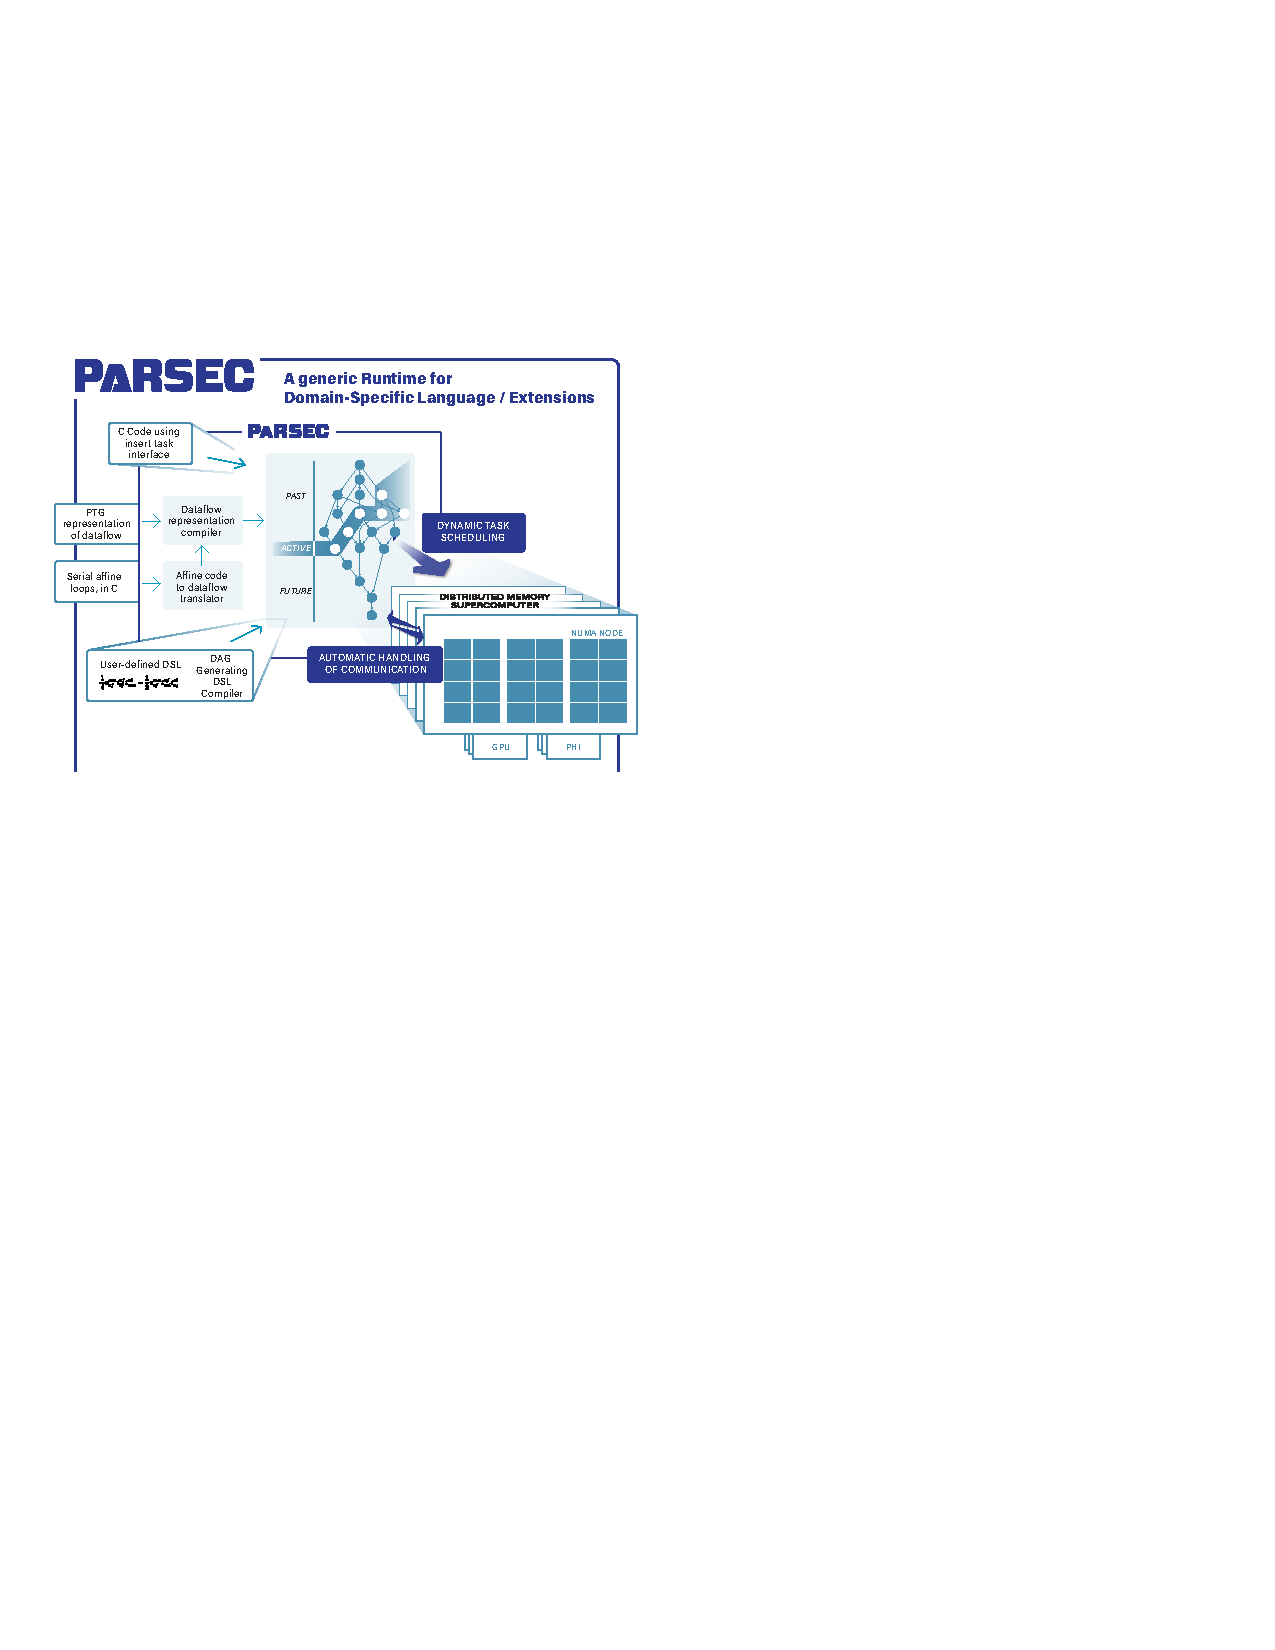
\includegraphics[width=\linewidth]{parsec.pdf}
%%     \end{center}
%%   \end{textblock*}
%% \end{frame}

%% \begin{frame}
%%   \frametitle{Performance Evaluation}

%%   Performance setup:
%%   \begin{itemize}
%%   \item Summit, $\approx$100 GPUs
%%   \item PaRSEC, with local iterators, NVlink support, GPU memory advice
%%   \item libDBCSR, master branch
%%   \end{itemize}

%%   Benchmarks:
%%   \begin{itemize}
%%   \item Synthetic benchmark: random sparsity, random tiling
%%     \begin{itemize}
%%     \item Tiling: average tile size of $1024\times 1024$
%%     \item smallest tile dimension: 512
%%     \item largest tile dimension: 2048
%%     \item[~]
%%     \item Sparsity: fill random (uniform) tiles in the matrix, one by one, until a threshold is reached
%%     \end{itemize}
%%   \item Applicative benchmark: $C_{65}H_{132}$, with 3 possible tilings
%%   \end{itemize}
  
%% \end{frame}

%% \begin{frame}
%%   \frametitle{Synthetic Benchmark}
%%   \relsize{-2}
%%   16 nodes of Summit -- 96 x V100 (GEMM peak: 672 TFlops/s)

%%   PaRSEC: 3 GPU / process, grid of $4\times 8$ processes

%%   libDBCSR: 1 GPU / process, tested all process grids, kept the best for each point
  
%%   \begin{center}
%%     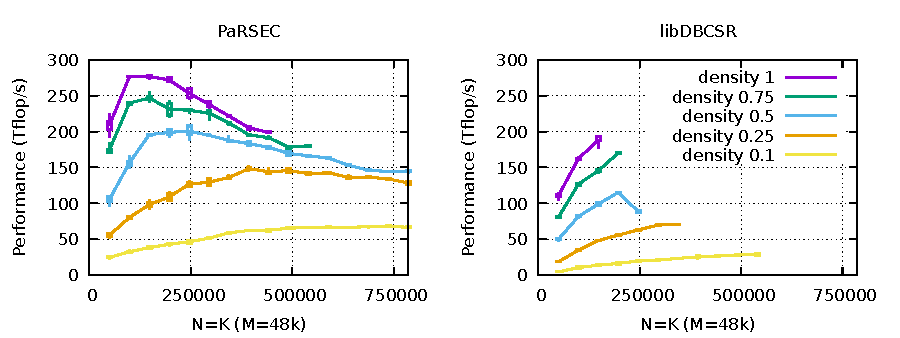
\includegraphics[width=.9\linewidth]{perf-synthetic.pdf}
%%   \end{center}

%%   \flushright\textcolor{orange}{Note: Evaluation stops when libDBCSR could not handle problem size}

%% \end{frame}

%% \begin{frame}
%%   \frametitle{Synthetic Benchmark}
%%   \relsize{-2}
%%   16 nodes of Summit -- 96 x V100 (GEMM peak: 672 TFlops/s)

%%   PaRSEC: 3 GPU / process, grid of $4\times 8$ processes

%%   \begin{columns}
%%     \begin{column}{.45\linewidth}
%%       \begin{center}
%%         Time to completion\\
%%         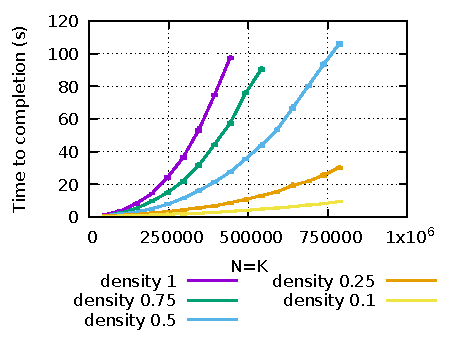
\includegraphics[width=.9\linewidth]{time-synthetic.pdf}
%%       \end{center}
%%     \end{column}
%%     \begin{column}{.45\linewidth}
%%       \begin{center}
%%         Arithmetic Intensity\\
%%         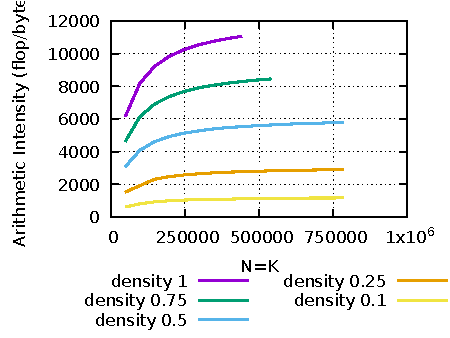
\includegraphics[width=.9\linewidth]{ai-synthetic.pdf}
%%       \end{center}
%%     \end{column}
%%   \end{columns}
%% \end{frame}

\begin{frame}
  \frametitle{$C_{65}H_{132}$}

  \begin{columns}
    \begin{column}{.35\linewidth}
      \begin{center}
        \relsize{-2}
        \begin{tabular}{cc}
          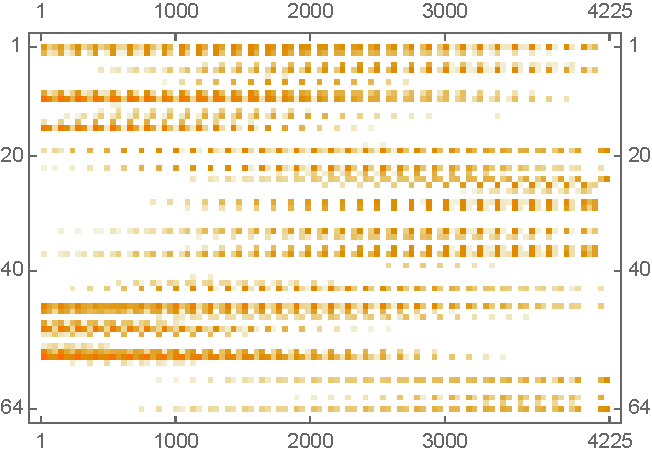
\includegraphics[width=0.45\linewidth]{t2_shape_v1.pdf} & 
          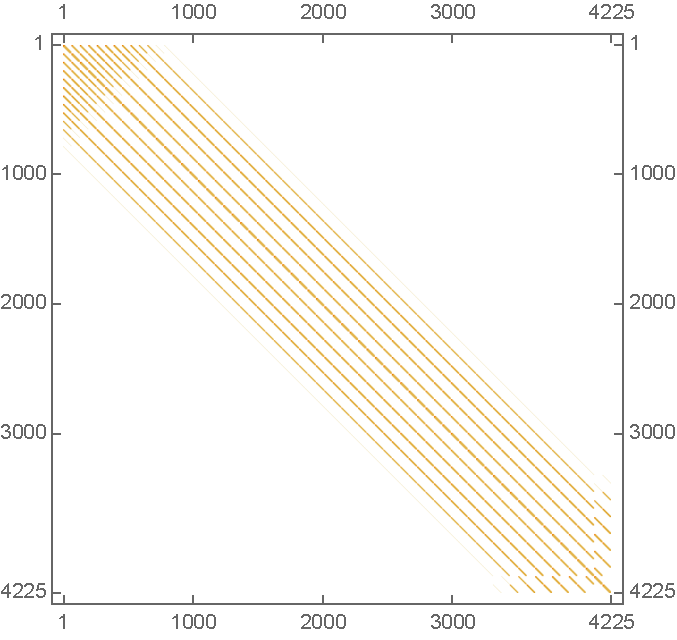
\includegraphics[width=0.45\linewidth]{v_shape_v1.pdf} \\
          $T$ & $V$ \\
          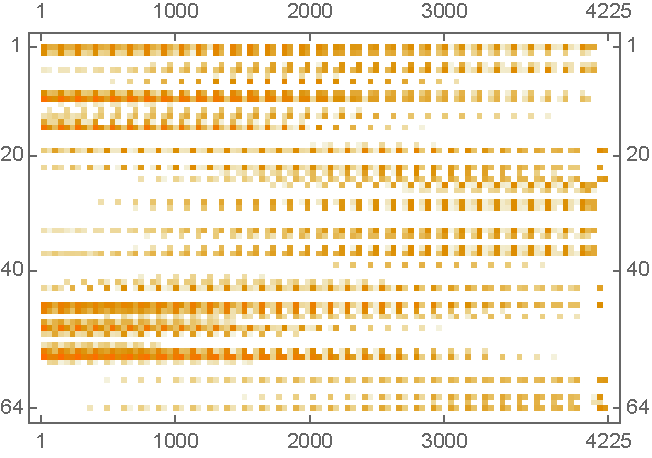
\includegraphics[width=0.45\linewidth]{r_shape_v1.pdf} & 
          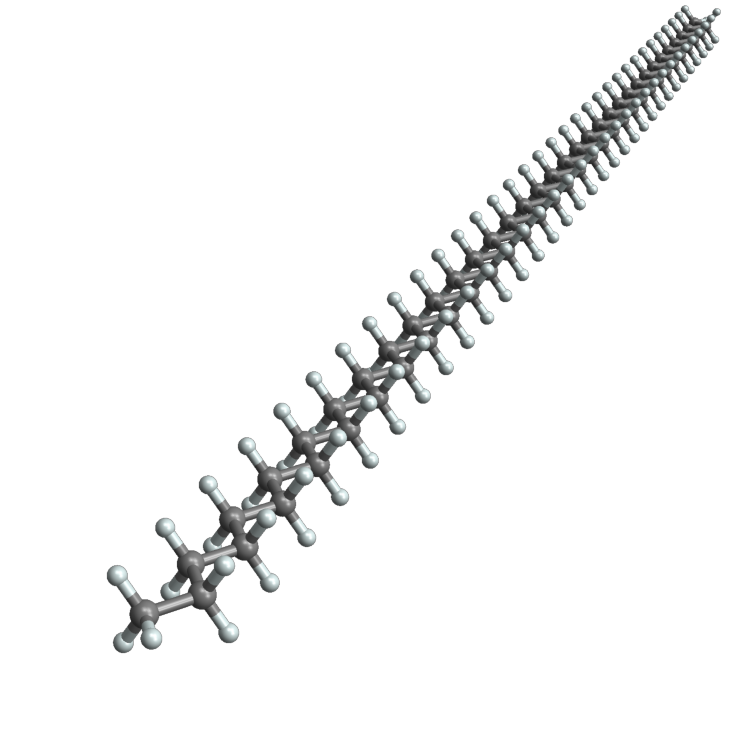
\includegraphics[width=0.45\linewidth]{c65h132.pdf} \\
          $R$ & the \ce{C65H132} molecule \\
        \end{tabular}
        (Tiling v1)
      \end{center}
    \end{column}

    \begin{column}{.5\linewidth}
      \relsize{-2}
      \begin{center}
        \begin{tabular}{l|l|l|l}
          & Tiling $v_1$ & Tiling $v_2$ & Tiling $v_3$ \\\hline
          $M\times N\times K$ & \multicolumn{3}{|c}{$26576\times 2464900 \times 2464900$} \\\hline
          \#flop & 877 Tflop & 923 Tflop & 1237 Tflop \\\hline
          \#flop (opt.) & 850 Tflop & 899 Tflop & 1209 Tflop \\\hline
          \#GEMM tasks & 1899971 & 468368 & 67818 \\\hline
          \#GEMM tasks (opt.) & 1843309 &455159& 66315 \\\hline
          Average \#rows/block & 700 & [500;2500] & [1000;5000]\\\hline
          Average \#col./block & 700 & [500;2500] & [1000;5000]\\\hline
          Density of $T$ & 9.8\% &  10.2\% & 13.2\%\\\hline
          Density of $V$ & 2.4\% & 2.6\% & 3.1\%\\\hline
          Density of $R$ (opt.) & 14.9\% & 16.1\% & 21.7\%\\
        \end{tabular}

        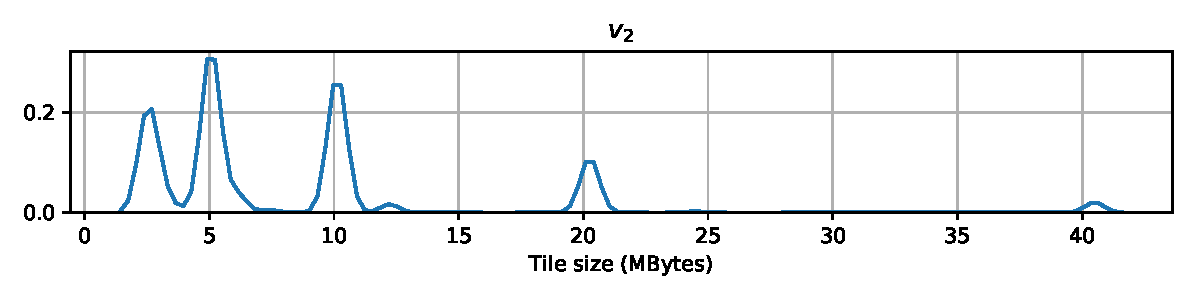
\includegraphics[width=\linewidth]{bs-distrib.pdf}
        
        (Tile size distribution for v2)
      \end{center}
    \end{column}
  \end{columns}
  
\end{frame}

\begin{frame}
  \frametitle{$C_{65}H_{132}$ Strong scaling}

  \begin{columns}
    \begin{column}{.45\linewidth}
      \begin{center}
        Time to completion
        
        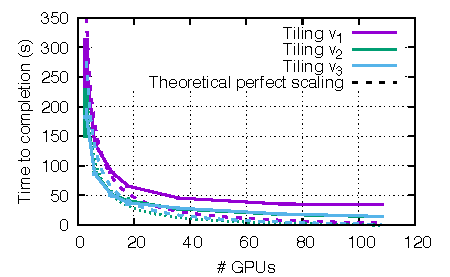
\includegraphics[width=\linewidth]{c65h132-time.pdf}
      \end{center}
    \end{column}
    \begin{column}{.45\linewidth}
      \begin{center}
        Performance
          
          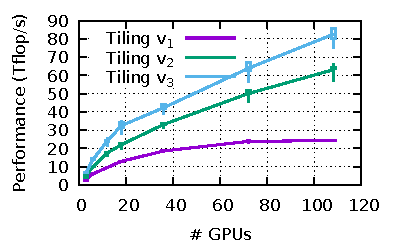
\includegraphics[width=\linewidth]{c65h132-perf.pdf}
      \end{center}
    \end{column}
  \end{columns}
\end{frame}

\begin{frame}
  \frametitle{Conclusion}

  Summary:
  \begin{itemize}
  \item Block-Sparse GEMM product, with irregular tiling, on distributed multi-GPUs, with problems that will not fit the GPU memory
  \item Tensor contraction, application in electronic structure computations
  \item Algorithm: placement of largest data, blocking per memory constraints
  \item Implementation: Problem-specific control flow on top of the basic block-sparse, irregularly tiled GEMM dataflow
  \item Performance: 2x libDBCSR on problems it can handle, can handle much bigger problems
  \item Performance: 35\% parallel efficiency, peak flop is limited by
    sparsity, time to solution less than a minute
  \end{itemize}

  Ongoing work:
  \begin{itemize}
  \item All algorithms of TiledArray (incl. ABCD) are being ported over TTG over PaRSEC
  \end{itemize}
  
\end{frame}

